\section{System}
\label{sec:sys}

Our \ql system implementation builds on Apache Spark with GraphX.  We
selected Spark because it is a popular open-source system, and because
of its in-memory processing approach.  All \tg operations are
available through the public API of the \ql library, and may be used
like any other library in an Apache Spark application.\eat{  \insql{TGraph}
is the main abstract class that all physical representations extend.
An excerpt of the API, where VD is the vertex attribute and ED is the
edge attribute type:}

\eat{\begin{lstlisting}
def slice(bound: Interval): TGraph[VD, ED]
def aggregate(window: WindowSpecification, vquant: Quantification, equant: Quantification, vAggFunc: (VD, VD) => VD, eAggFunc: (ED, ED) => ED)(vgroupby: (VertexId, VD) => VertexId): TGraph[VD, ED]
def union(other: TGraph[VD, ED]): TGraph[Set[VD], Set[ED]]
\end{lstlisting}}

\subsection{Physical Representations}
\label{sec:sys:datastructs}

We considered four in-memory \tg representations that differ both in
compactness and in the kind of locality they prioritize. With {\em
  structural locality}, neighboring vertices (resp. edges) of the same
representative graph are laid out together, while with {\em temporal
  locality}, consecutive states of the same vertex (resp. edge) are
laid out together~\cite{DBLP:journals/tos/MiaoHLWYZPCC15}.  We now
describe each representation.\eat{ VertexEdge (VE) is a direct
  translation of the \ve model of Definition~\ref{def:tg_ve} and the
  most compact representation.  While VE does not necessitate a
  particular order of tuples on disk, we opt for a physical layout in
  which all tuples corresponding to the same vertex (resp. edge) are
  laid out consecutively, and so VE preserves temporal locality.
  RepresentativeGraphs (RG) directly implements the data structure of
  Definition~\ref{def:tg_abstract}, storing each representative graph
  explicitly, and so naturally preserves structural locality, but
  temporal locality is lost.  OneGraph (OG) stores all vertices and
  edges of an evolving graph once, in a single data structure.  This
  representation emphasizes temporal locality, while also preserving
  structural locality.  HybridGraph (HG) trades compactness for better
  structural locality, by aggregating together several consecutive
  RGs, and computing a OneGraph for each RG group.  Details of our
  implementation of the four representations are given below.}

\eat{\reminder{Support experimentally or remove / rephrase: We can convert
  from one representation to any other at small or no cost, so it is
  useful to think of them as access methods in the context of
  individual operations.}}

\eat{
\begin{table*}[t]
\centering
\small
\begin{tabular}{ p{1.6cm} | p{3.5cm} | p{3.5cm} | p{3.5cm} | p{3.5cm} }
\hline
\multicolumn{1}{l|}{\bfseries Operation} & \multicolumn{1}{c|}{\bfseries VE} & \multicolumn{1}{c|}{\bfseries RG} & \multicolumn{1}{c|}{\bfseries OG} & \multicolumn{1}{c|}{\bfseries HG} \\ \hline
slice & filter V and E; modify periods to be within slice interval & slice sequence of RGs & filter indices in bitsets & slice sequence of OGs and filter indices in remaining OGs \\ \hline
select & filter V ad E; enforce FK constraint & only when predicate not on interval: filter V and E of each RG & N/A & N/A \\ \hline
project & apply projection to each element of defined projection; coalesce & apply projection to each element within each RG; coalesce and recompute & N/A & N/A \\ \hline
aggregate (non-structural) & split each vertex/edge by window; reduce by window key; filter those under quantification threshold; enforce FK constraint & map each RG to windows; group vertices/edges in each window into one RG, filtering by quantification & only structure: for each vertex/edge map indices in bitsets to corresponding windows; filter by quantification threshold; enforce FK constraint & only structure: combine OGs as necessary to group into windows; map indices in bitsets; filter by quantification threshold; enforce FK constraint \\ \hline
aggregate (with structural) & map each vertex to new id; join edges with new vertices to get new id; rest as above & within each window map vertices and edge triplets to new ids; rest as above & N/A & N/A \\ \hline
union & compute combined intervals; split each vertex/edge by new intervals; full outer join & compute combined intervals; combine RGs in corresponding intervals; full outer join & structure only: remap bitsets to new intervals; union vertices/edges from two graphs and reduce by key to combine bitsets & structure only: combine OGs as necessary; rest as in OG \\ \hline
intersection & compute intervals; split each vertex/edge by new interval; inner join & compute intervals; inner join of vertices/edges from corresponding intervals & structure only: like union but with bitset intersection & structure only: like union but with bitset intersection \\ \hline
analytics (pagerank, shortest paths, etc.) & N/A & compute for each RG & compute for all periods simultaneously & compute for all periods within each OG simultaneously \\ 
\hline
\end{tabular}
\caption{Operations.}
\label{tab:operations}
\end{table*}
}

{\bf RepresentativeGraphs (RG)} is a direct implementation of \trg of
Definition~\ref{def:tg_abstract}.  RG is a collection (parallel
sequence) of GraphX graphs, where vertices and edges store the
attribute values for the specific time interval, thus using structural
locality.  This representation supports all operations of \tg algebra.
%
While the \rg representation is simple, it is not compact, considering
that in many real-world evolving graphs there is a 80\% or larger
similarity between consecutive
snapshots~\cite{DBLP:journals/tos/MiaoHLWYZPCC15}.  In a distributed
architecture, however, this data structure provides some benefits as
operations on it can be easily parallelized by assigning different
representative graphs to different workers.

\rg is the most immediate way to implement evolving graphs using
GraphX. Without \ql a user wishing to analyze evolving graphs might
implement and use the \rg approach.  However, as we will show in
Section~\ref{sec:exp}, this would lead to poor performance for most
operations.

\begin{figure}[t!]
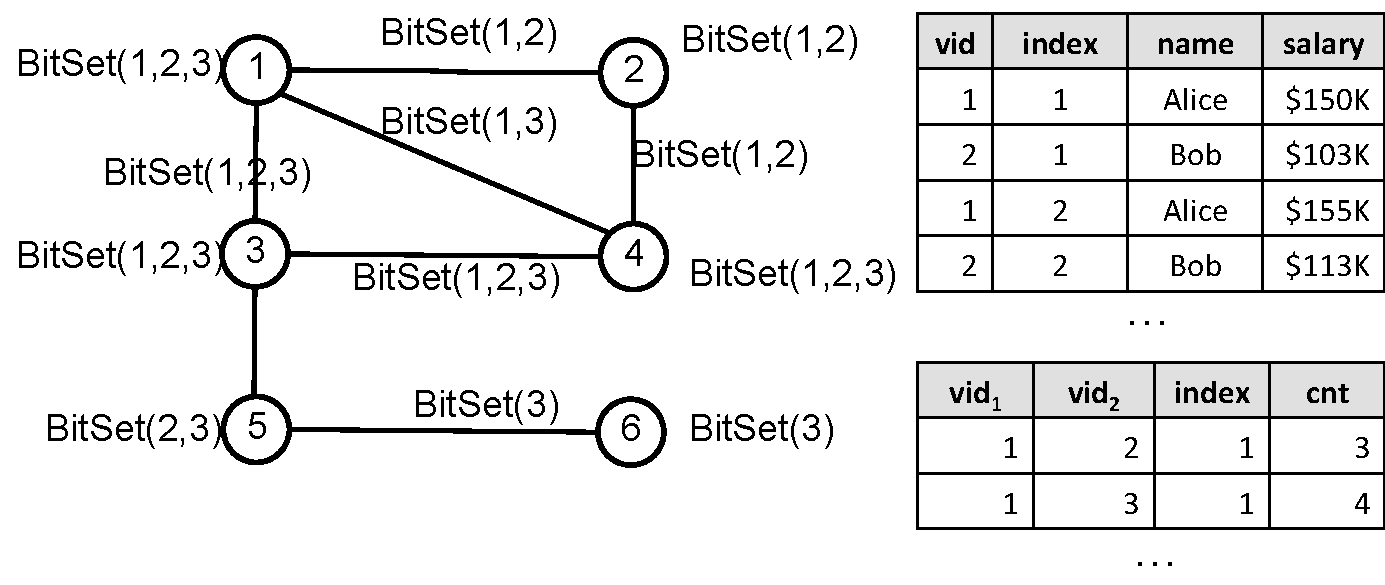
\includegraphics[width=3in]{figs/ogc.pdf}
\caption{\og representation of \insql{T1}.}
\label{fig:ogc}
\end{figure}

{\bf VertexEdge (VE)} is a direct implementation of the \tve model of
Definition~\ref{def:tg}, and is the most compact: one RDD contains all
vertices and another all edges.  Consistently with the GraphX API, all
vertex properties are stored together as a single nested attribute, as
are all edge properties.  We currently do not store the \tv and \te
relations separately but rather together with \tav and \tae,
respectively.  While VE does not necessitate a particular order of
tuples on disk, we opt for a physical layout in which all tuples
corresponding to the same vertex (resp. edge) are laid out
consecutively, and so VE preserves temporal localilty.

\eat{ The main advantage of this schema-less attribute representation
  is that it can easily deal with schema evolution and leaves the
  details of attribute processing to the user. } 

The VE representation supports all \tg algebra operations but cannot
support analytics.  This is because an analytic is defined on a
representative graph, which VE does not materialize.  As we will show
in Section~\ref{sec:exp}, due to compactness this physical
representation is the most efficient for many operations.

{\bf OneGraph (OG)} is the most topologically compact representation,
which stores all vertices from \tav {\em and} edges from \tae once, in
a single data structure.  Information about time validity is stored
together with each vertex and edge.  Figure~\ref{fig:ogc} shows the OG
for \insql{T1} from Figure~\ref{fig:tg_rg}.  OG emphasizes temporal
locality, while also preserving structural locality, but leads to a
much denser graph than RG.  This, in turn, makes parallelizing
computation challenging.

An OG is implemented as a single GraphX graph.  To construct an \og
from \tve, vertices and edges of \tv and \te relations each are
grouped by key and mapped to bitsets, which in turn encode the
presence of a vertex or edge in each time period associated with some
representative graph of a \tg.  Because \og stores information only
about graph topology, far fewer periods must be represented and
computed for \og than for \rg.  The actual reduction depends on the
rate and nature of graph evolution.

As we will see experimentally in Section~\ref{sec:exp}, \og is often
the best-performing data structure for aggregation, and also has
competitive performance for analytics.  Because of this focus, \og
supports operations only on topology: analytics, aggregation. union,
and intersection for graphs with no vertex or edge attributes.  For
completeness, all other operations are supported through inheritance
from an abstract parent, and are carried out on the VE data structure.

{\bf HybridGraph (HG)} trades compactness of \og for getter structural
locality of \rg, by aggregating together several consecutive
representative graphs, computing a single \og for each graph group,
and storing these as a parallel sequence.  In our current
implementation each \og in the sequence corresponds to the same number
of temporally adjacent graphs.
%
This is the simplest grouping method, and we observed that placing the
same number of graphs into each group often results in unbalanced
group sizes.  This is because evolving graphs commonly exhibit strong
temporal skew, with later graphs being significantly larger than earlier
ones.  We are currently working on more sophisticated grouping
approaches that would lead to better balance, and ultimately to better
performance.  However as we will see experimentally in
Section~\ref{sec:exp}, the current \hg implementation already improves
performance compared to \og, in some cases significantly.

Like \og, the \hg representation focuses on topology-based analysis,
and so does not represent vertex and edge attributes. OG implements
analytics, aggregation, union, and intersection, and supports all
other operations through inheritance from VE.

%\section{Lazy Coalescing}
\subsection{Lazy Coalescing}
\label{sec:sys:coal}

\eat{
\begin{table}
\small
\begin{tabular}{ l | p{4cm} | c }
\hline
\multicolumn{1}{l|}{\bfseries Operation} & \multicolumn{1}{c|}{\bfseries Requires Coalesced Input} & \multicolumn{1}{c}{\bfseries Uncoalesces} \\ \hline
slice & no & no \\ \hline
select & only if predicate incl. interval & no \\ \hline
project & no & yes \\ \hline
aggregate & only if structural group by is used and includes interval & yes \\ \hline
union & no & yes \\ \hline
intersection & no & yes \\ \hline
analytics & no & yes \\
\hline
\end{tabular}
\caption{Coalesce analysis.}
\label{tab:coalesce}
\end{table}
}

All operations and all sequences of operations must output a valid
temporally coalesced \tg.  Several implementations are possible for
the coalesce operation over temporal SQL relations,
see~\cite{DBLP:conf/vldb/BohlenSS96} for details.  We use the
partitioning method, where the relation (e.g., \tv, \te, \trg) is
grouped by key, and tuples are sorted and folded within each group to
produce time periods of maximum length.  This involves shuffling
between partitions, is computationally expensive, and motivates
lazy coalescing.

Correctness of many \tg algebra operations does not depend on whether
their input is coalesced.  Consequently, \ql supports both eager and
lazy coalescing, with lazy being the default for queries that admit
it.  We now present useful coalescing rules.

\eat{ As with duplicate elimination, if the coalesced output is
  expected to be significantly reduced in size, such as after a
  project operation on a high volatility attribute, performing
  coalesce eagerly before a time-consuming operation, especially
  analytics, can be advantageous.}
%

\eat{{\bf Successive coalescing is unnecessary} in \tg algebra just as it
is for (non-graph) temporal
databases~\cite{DBLP:conf/vldb/BohlenSS96}:}
\eat{\begin{equation}
\cl(\cl(\ttt)) \equiv \cl(\ttt)
\label{rul:twice}
\end{equation}}

\eat{It is unnecessary to coalesce an already coalesced \ttt, e.g., if the
data on disk is known to be coalesced:}

\eat{\begin{equation} 
\cl(\ttt) \equiv \ttt~~\text{iff}~\textsf{is\_coalesced}(\ttt)
\label{rul:cond}
\end{equation}}

%The first rule eliminates successive coalescing:

%\begin{equation}
%\cl(\cl(\ttt)) \equiv \cl(\ttt)
%\label{rul:coalr0}
%\end{equation}

{\bf Slice allows lazy coalescing.}  We showed in
Section~\ref{sec:algebra:slice} that slice does not destroy
coalescing.  Further, recall that $\tau_c(\cl(\ttt))$ returns tuples
$(x,p \cap c)$, for which $p \cap c \neq \emptyset$.  If \ttt is
uncoalesced, then there exist some value-equivalent tuples $(x, p_1)$
and $(x, p_2)$
s.t. $\pred{p_1}{meets}{p_2}~\lor~\pred{p_1}{contains}{p_2}~\lor$\\$\pred{p_1}{overlaps}{p_2}$,
which would be replaced by $(x, p_1 \cup p_2)$ in \cl(\ttt).  Because
intersection distributes over union, i.e.,$(p_1 \cup p_2) \cap c =
(p_1 \cap c) \cup (p_2 \cap c)$, coalescing can be equivalently
performed before or after slice: \eat{$\cl(\tau_c(\ttt)) \equiv
\tau_c(\cl(\ttt))$.}
\begin{equation}
\cl(\tau_c(\ttt)) \equiv \tau_c(\cl(\ttt))
\label{rul:slice}
\end{equation}

{\bf Temporal subgraph may allow lazy coalescing.} It was shown
in~\cite{DBLP:conf/vldb/BohlenSS96} that coalescing can be deferred
until after selection if the selection condition is independent of the
valid time of the input. If temporal subgraph
(Section~\ref{sec:algebra:subgraph}) is time-invariant, coalescing can
be deferred.  \eat{Subgraph does not uncoalesce \tve but may
  uncoalesce \trg (Section~\ref{sec:algebra:subgraph}). For this
  reason it is required to coalesce the final output in
  Rule~\ref{rul:subgraphrg} even if the input was eagerly coalesced,
  but this is not required in Rule~\ref{rul:subgraphve}.}
\begin{multline}
\cl(\sigma_{C_V,C_E}(\ttt)) \equiv \sigma_{C_V,C_E}(\cl(\ttt))\\ \text{iff } independent\_of\_p(C_V) \wedge independent\_of\_p(C_E)
\label{rul:subgraphve}
\end{multline}
\eat{\begin{equation}
\cl(\sigma_{C_V,C_E}(\trg)) \equiv \cl(\sigma_{C_V,C_E}(\cl(\trg)))
\label{rul:subgraphrg}
\end{equation}}

Deferring coalescing can be quite effective for Rules~\ref{rul:slice}
and ~\ref{rul:subgraphve} if the selectivity of the predicate is high.

{\bf Temporal map may allow lazy coalescing}, since it processes each
input tuple without modifying the corresponding time intervals, as
long as it is time-invariant.  Map destroys coalescing
(Section~\ref{sec:algebra:project}), and requires to coalesce the
output even if the input was eagerly coalesced.
\begin{multline}
\cl(\map_{M_V,M_E}(\ttt)) \equiv \cl(\map_{M_V,M_E}(\cl(\ttt)))\\ \text{iff } independent\_of\_p(M_v) \wedge independent\_of\_p(M_E)
\label{rul:map}
\end{multline}

\eat{Rules in ~\ref{rul:coalr1,rul:coalr2,rul:coalr3} exploit the fact that
some operations preserve coalescing, as shown in
Section~\ref{sec:algebra}:}

\eat{\begin{equation}
coal(\tau_c(coal(T))) \equiv \tau_c(coal(T))
\label{rul:coalr1}
\end{equation}
\begin{equation}
coal(\sigma_f(coal(\tve))) \equiv \sigma_f(coal(\tve))
\label{rul:coalr2}
\end{equation}
\begin{equation}
coal(udf(coal(T))) \equiv udf(coal(T))
\label{rul:coalr3}
\end{equation}}

\eat{Rules in
~\cref{rul:coalr4,rul:coalr5,rul:coalr6,rul:coalr7,rul:coalr8,rul:coalr9}
cover operations which are invariant with respect to time and so
coalescing can be postponed until after the operation:}

\eat{\begin{equation}
\tau_c(coal(T)) \equiv coal(\tau_c(T))
\label{rul:coalr4}
\end{equation}}

\eat{Recall that slice selects each entity with an interval that intersects
with $c$ and modifies only the selected tuple periods to $p \cap c$.
According to the rule~\ref{rul:coalr1}, slice does not uncoalesce.  If
the input relation is uncoalesced, it contains some value-equivalent
tuples with adjacent or overlapping periods.  According to the
definitions of $intersect$ and $coalesce$, an intersect with interval
$p$ is the same as the coalesce of intersects of intervals composing
$p$.  I.e., $p \cap c = (p1 \cap c) \cup (p2 \cap c$) where $p = p1
\cup p2$.  Thus coalescing can be performed before or after slice.}

\eat{\begin{equation}
coal(\sigma_f(coal(T))) \equiv coal(\sigma_f(T))
\label{rul:coalr5}
\end{equation}}

\eat{As shown in~\cite{DBLP:conf/vldb/BohlenSS96}, coalescing can be
deferred until after the selection if the selection condition is
independent of the valid time of the input. Since subgraph is a
time-invariant form of select, coalesce is not required prior to
subgraph.  For both this rule and the slice rule above, deferring
coalescing can be quite effective if the selectivity of the predicate
is high.}

\eat{\begin{equation}
coal(\mu(coal(T))) \equiv coal(\mu(T))
\label{rul:coalr6}
\end{equation}}

\eat{The map operation processes each tuple without modifying the
corresponding intervals and independently of the valid time of the
input.  Thus, as above, coalesce can be deferred.}

\eat{\begin{equation}
coal(coal(T_1) \cap coal(T_2)) \equiv coal(T_1 \cap T_2)
\label{rul:coalr7}
\end{equation}}

\eat{\begin{equation}
coal(coal(T_1) \cup coal(T_2)) \equiv coal(T_1 \cup T_2)
\label{rul:coalr8}
\end{equation}}

\eat{For \trg, temporal graph intersection is a inner theta-join followed
by projection.  As shown in~\cite{DBLP:conf/vldb/BohlenSS96},
coalescing can be deferred until after a join and after a projection
if that projection is independent of the valid time interval of the
tuple, which is the case here.  Thus we can defer coalescing until
after the temporal graph intersection.  Temporal graph union is also a
join, albeit an outer one, so the same argument applies.}

\eat{\begin{equation}
coal(udf(coal(T))) \equiv coal(udf(T))
\label{rul:coalr9}
\end{equation}}

{\bf Temporal aggregation requires eager coalescing.}  When
aggregating by change, the input must be coalesced to compute correct
aggregation windows.  If the input is not coalesced, then there may be
two or more consecutive intervals which should be treated as one but
would count separately. For aggregation by time, some aggregate
functions also require coalesced input.  For example, \insql{count}
will produce different result if several consecutive or overlapping
value-equivalent tuples fall within the same window.  Thus we add the
following conditional coalescing rule:
\begin{fleqn}[0pt]
\begin{multline}
\cl(\gamma_{W,Q_V,Q_E,A_V,A_E}(\cl(\ttt))) \equiv \cl(\gamma_{W,Q_V,Q_E,A_V,A_E}(\ttt)) \\
\text{iff}~~W \text{by\_time} \wedge A_V, A_E \in \{\insql{any},\insql{first}, \insql{last},\insql{min}, \insql{max} \}
\label{rul:agg}
\end{multline}
\end{fleqn}

\insql{any} returns any one of the values associated with a property
within each group in $W$, and so is invariant to time and to the
number of tuples in $W$.  \insql{first} and \insql{last} pick the
earliest (resp. latest) value within each group in $W$.  If \ttt is
uncoalesced, there is at least one pair of value-equivalent tuples
with overlapping or consecutive periods.  Selecting between equivalent
values will generate the same result.  The same argument applies to
\insql{min} and \insql{max}.

{\bf Temporal intersection and union allow lazy coalescing.} For \trg,
temporal graph intersection (Section~\ref{sec:algebra:join}) is a join
followed by projection.  As shown in~\cite{DBLP:conf/vldb/BohlenSS96},
coalescing can be deferred until after a join, and after a projection
if projection is independent of the valid time interval of the tuple,
which is the case here.  Thus we can defer coalescing until after
temporal graph intersection.  Temporal graph union
(Section~\ref{sec:algebra:outerjoin}) is an outer join, and the same
argument applies.  Note that both operations may destroy coalescing,
and so a final coalesce is required over the result even if inputs
were eagerly coalesced.
\begin{equation}
\cl(\cl(\ttt_1) \cap \cl(\ttt_2)) \equiv \cl(\ttt_1 \cap \ttt_2)
\label{rul:intersect}
\end{equation}
\begin{equation}
\cl(\cl(\ttt_1) \cup \cl(\ttt_2)) \equiv \cl(\ttt_1 \cup \ttt_2)
\label{rul:union}
\end{equation}

{\bf Temporal user-defined analytics allow lazy coalescing.} If \trg
is not coalesced, it contains one or more value-equivalent
representative graphs with consecutive or overlapping periods.
Analytics are time-invariant functions applied to each representative
graph.  Thus when applied to value-equivalent graphs, they will
produce equivalent results, and so coalesce can be deferred.  Further,
analytics to not destroy coalescing, and so it is not required to
coalesce again over the final result.  
\begin{equation}
\cl(\uda(\ttt)) \equiv \uda(\cl(\ttt))
\label{rul:analytic}
\end{equation}
Although it is possible to defer coalesce for analytics, this will not
be done in practice.  Analytics are computationally expensive, and it
is usually beneficial to eagerly coalesce the input, reducing the
number of representative graphs.

%Finally, a rule that eliminates coalescing of coalesced \tgs:

\eat{\begin{equation}
coal(T) \equiv T~~iff~~is\_coalesced(T)
\label{rul:coalr11}
\end{equation}}

%This last rule is very useful if the data on disk is known to be
%coalesced.



\subsection{Implementation}
\label{sec:sys:maint}

{\bf Enforcing referrential integrity.}  The \tve representation of a
\tg (Definition~\ref{def:tg}) requires that referrential integrity be
maintained by algebraic operations, and this is done on lines 6---8 of
Algorithm~\ref{alg:op}.  In Section~\ref{sec:algebra} we discussed
that temporal subgraph~\ref{sec:algebra:subgraph} and
aggregation~\ref{sec:algebra:agg} both require that tuples be removed
from \te, or that their periods of validity be modified to be included
within the periods of validity of the corresponding vertices
(Condition~\ref{def:tg:c1} of Definition~\ref{def:tg}), due to changes
in \tv.  We do this by executing a join of \te with \tv on vertex ids
--- either a broadcast join if \tv is small, or a hash join --- and
then adjusting time periods as necessary.  This is an expensive
operation and is only performed when necessary: when temporal subgraph
has a non-trivial predicate on $C_V$, and when temporal aggregation
has a more restrictive vertex aggregation quantifier $Q_V$ than edge
quantifier $Q_E$ (see the end of Section~\ref{sec:algebra:agg} for a
discussion).

\julia{Vera: is this still relevant?  What does this mean? ``GraphX
  graphs maintain foreign key constraint during subgraph operation and
  we make use of this for all physical representations besides VE.''}

  \eat{
    {\bf Foreign key constraint.}  The \ve data model includes a
    foreign key constraint from edges to vertices.  This constraint is
    naturally maintained by most operations while performing
    operations on V and E independently, as shown in
    Section~\ref{sec:algebra}.  For \insql{subgraph} and
    \insql{aggregate} additional steps are required to insure
    correctness.  We modify E tuples to enforce the foreign key
    constraint by joining on V, using either a broadcast or hash join
    depending on the size of V.  Each edge period is then modified to
    be the overlap of the periods of source and destination vertices
    and the original edge period.  Because this step is
    computationally expensive, it is only taken when necessary: when
    \insql{subgraph} has a predicate on V and when \insql{aggregate}
    has a higher level of quantification for V than for E.  GraphX
    graphs maintain foreign key constraint during subgraph operation
    and we make use of this for all representations besides VE.}

{\bf Partitioning.}  Graph partitioning can have a tremendous impact
on system performance.  A good partitioning strategy needs to (1) be
balanced, assigning an approximately equal number of units to each
partition, and (2) limit the number of cuts across partitions, to
reduce cross-partition communication.  In our experiments we compare
performance with (1) no repartitioning after load, and (2) with
repartitioning using the 2D edge partitioning strategy (E2D).  This
strategy is available in GraphX and was used without modification.  In
E2D, a sparse edge adjacency matrix is partitioned in two dimensions,
guaranteeing a $2 \sqrt{n}$ bound on vertex replication, where $n$ is
the number of partitions. As has been shown
previously~\cite{DBLP:conf/osdi/GonzalezXDCFS14,MoffittTempWeb16}, E2D
provides good performance for Pregel-style analytics.

{\bf Graph loading.}  We use the Apache Parquet for storing our data
on disk, one archive for vertices and another for edges, temporally
coalesced.  This is a direct physical translation of the vertex-edge
\tg logical data model where the attributes are stored with the
topology.  In cases where there is 0 or 1 attribute per node/edge,
such as in our datasets, this is also the most compact representation.
If the input data is in uncoalesced snapshots, then it occupies space
as a function of the graph evolution rate.

For ease of use, we provide a GraphLoader utility that can initialize
any of the 4 physical representations of the \tg from Apache Parquet
files on HDFS or on local disk, provided they follow the correct
schema, using function call
\insql{GraphLoader.loadDataParquet(\$path)}.  The \ql user can also
write their own custom graph loading code to load vertices and edges
and then use \insql{fromRDDs} method to initialize any of the 4
representations.

\eat{ We have shown how our logical data model and semantics can be
  implemented in a distributed context. } While further implementation
details are out of the scope of this paper, the \ql code is freely
available online.  In the next section we show how different physical
representations behave on each operation.

